\subsection{Парабола}

{\bfseries \term{Парабола}} --- геометрическое место точек, равноудалённых от данной прямой (называемой \term{директрисой} параболы) и данной точки (называемой \term{фокусом} параболы).

{\itshape Каноническое уравнение параболы} имеет следующий вид:
\begin{equation}
y^2=2px,
\end{equation}
где $p$ --- \term{фокальный параметр}, равный расстоянию между фокусом параболы и директрисой или удвоенному расстоянию между фокусом параболы и вершиной.

Парабола в полярной системе координат $(\rho,\varphi)$ с центром в фокусе и нулевым направлением вдоль оси параболы (от фокуса к вершине) может быть представлена в виде уравнения
\begin{equation}
\rho(1+\cos\varphi)=p
\end{equation}

Эксцентриситет параболы равен $e=1$.
Важно отметить, что парабола не имеет \term{большой} и \term{малой полуоси}.

\begin{figure}[h!]
\centering
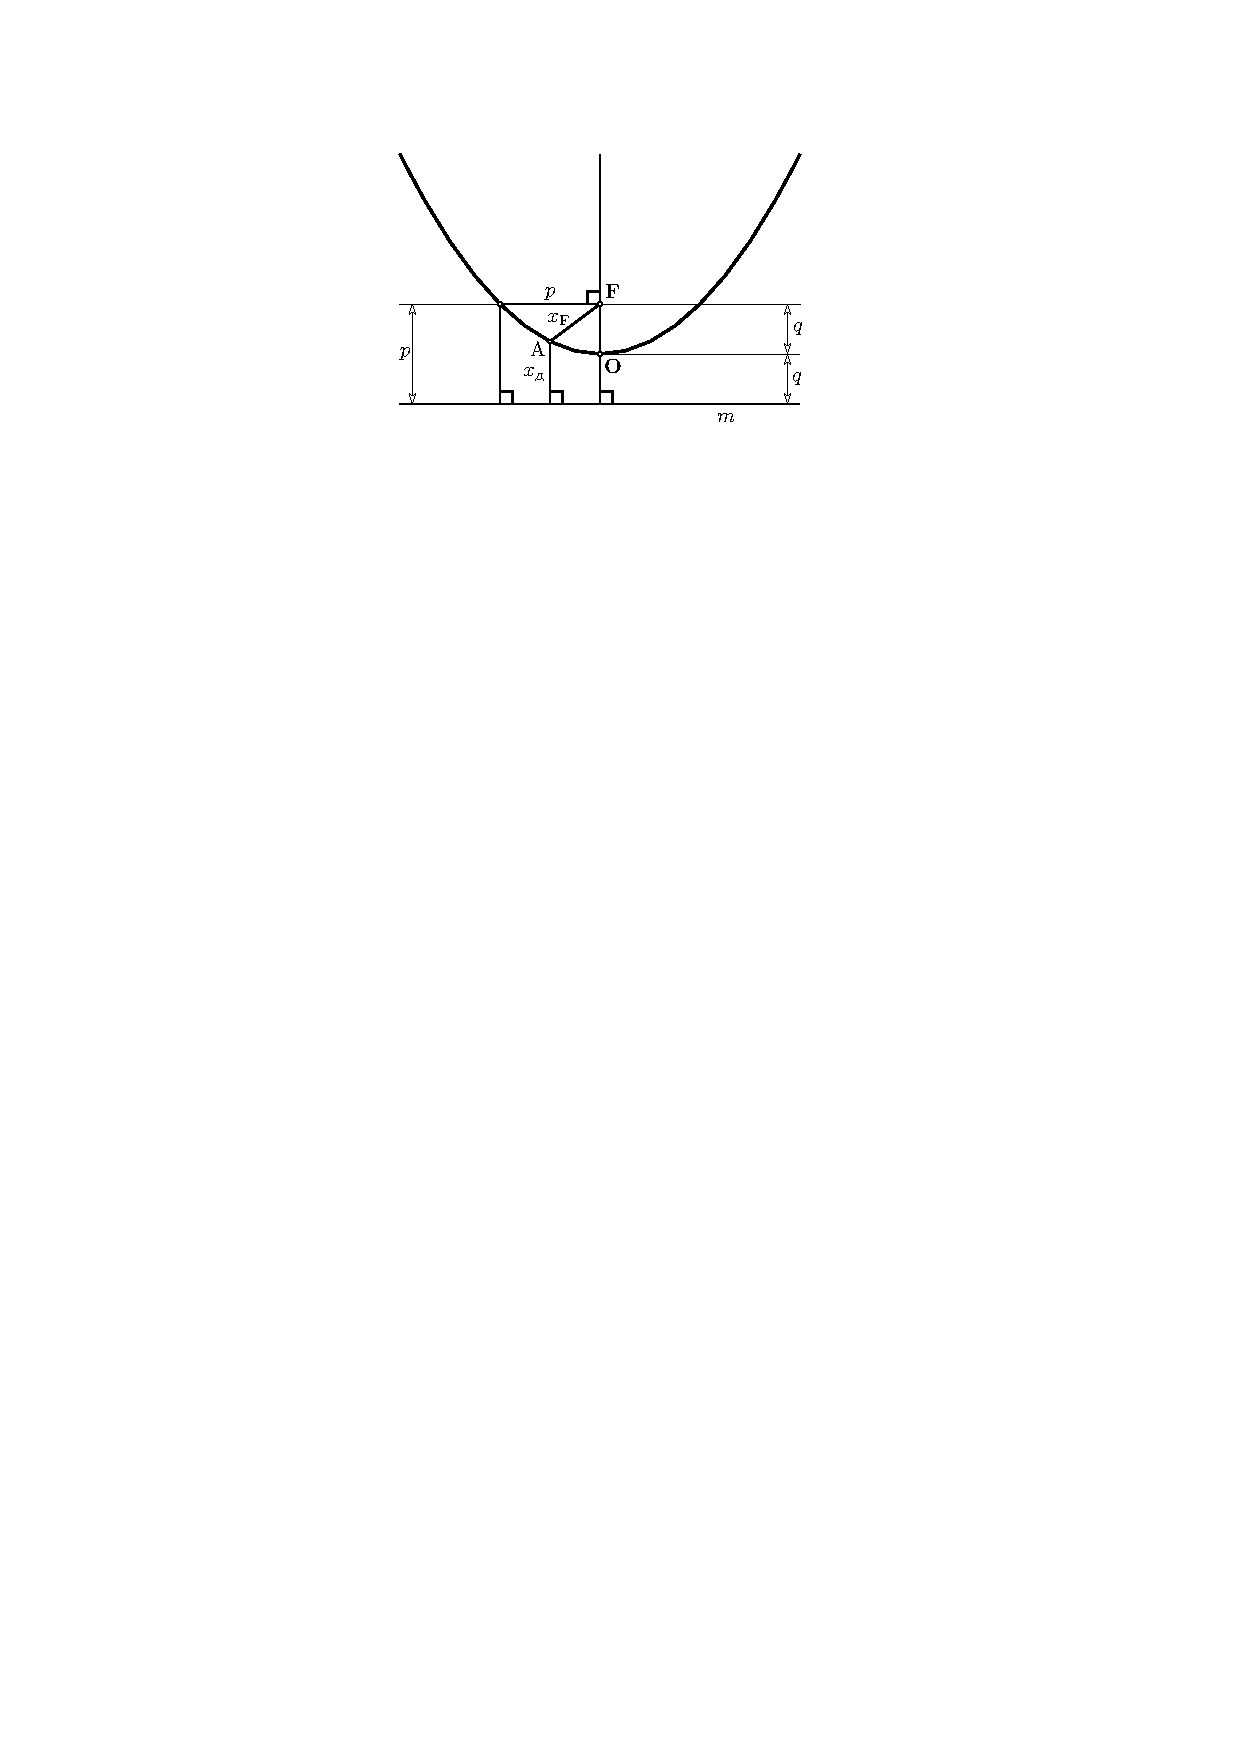
\includegraphics[width = 0.8\textwidth]{Parabola}
\caption{Парабола \label{pic:the-pic}}
\end{figure}

Как и все конические сечения, парабола обладает \textit{оптическим свойством}, которое формулируется следующим образом: пучок лучей, параллельных оси параболы, отражаясь в параболе, собирается в её фокусе. И наоборот, свет от источника, находящегося в фокусе, отражается параболой в пучок параллельных её оси лучей.

